\documentclass{standalone}
\usepackage{tikz}
\begin{document}
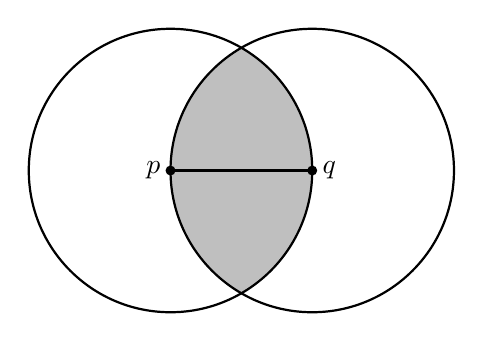
\begin{tikzpicture}[thick, scale=0.45]
\begin{scope}
\clip (-2,0) circle (4cm);
\clip (2,0) circle (4cm);
\fill[color=gray!50] (-4,4) rectangle (4,-4);
\end{scope}

\draw (-2,0) circle (4cm);
\draw (2,0) circle (4cm);
    
\path (-2, 0) coordinate [label= left:$p$] (p);
\path (2,0) coordinate  [label= right:$q$] (q);
\draw (p) -- (q);
    
\fill [black] (p) circle (4pt);
\fill [black] (q) circle (4pt);
\end{tikzpicture}
\end{document}